\input{../ee122.tex}
\usepackage{amsmath, dsfont, tikz, float}
\usepackage{graphicx}

\usetikzlibrary{arrows,automata,positioning}

\oddsidemargin 0in
\evensidemargin 0in
\textwidth 6.5in
\topmargin -0.5in
\textheight 9.0in

\newenvironment{amatrix}[1]{%
  \left(\begin{array}{@{}*{#1}{c}|c@{}}
}{%
  \end{array}\right)
}

\makeatletter
\renewcommand*\env@matrix[1][*\c@MaxMatrixCols c]{%
  \hskip -\arraycolsep
  \let\@ifnextchar\new@ifnextchar
  \array{#1}}
\makeatother

\newcommand{\norm}[1]{\left\lVert #1 \right\rVert}
\newcommand{\?}{\stackrel{?}{=}}
\newcommand\given[1][]{\:#1\vert\:}


\begin{document}

\solution{Nikhil Unni}{HW4}{Spring 2016}
\pagestyle{myheadings}

\begin{enumerate}
  \item Since A is actively communicating with B, E has received A's RTS towards B, and knows not to transmit, or else it will disturb A. Similalrly, C knows not to broadcast as well. So that just leaves:
    $$D \rightarrow E$$
    and
    $$D \rightarrow C$$

  \item Without RTS/CTS, the total time should be:
    $$\text{DIFS + backoff + overhead/payload + SIFS + ACK}$$
    And with RTS/CTS, the total time should be:
    $$\text{DIFS + backoff + RTS + SIFS + CTS + SIFTS + overhead/payload + SIFS + ACK}$$
    Actually plugging in the numbers, we know that :
    $$\text{DIFS } = 2.5(20 \mu s) = 50 \mu s$$
    $$\text{SIFS } = 0.5(20 \mu s) = 10 \mu s$$
    $$\text{RTS = CTS = ACK } = 10(20 \mu s) = 200 \mu s$$
    The transmission time of just the actual payload is:
    $$= \text{overhead + payload transmission time } = 9(20 \mu s) + X \text{ bytes} * \frac{1 \text{ bit}}{8 \text{ bytes}} * \frac{1s}{11,000,000 \text{ bits}} * \frac{1000000 \mu s}{1 s}$$
    $$= (180 + \frac{X}{88}) \mu s$$

    That means that the first (without RTS/CTS) backoff time should be $1.5(180 + \frac{X}{88}) \mu s$, and the second backoff time should be $1.5(200 \mu s) = 300 \mu s$.

    So the transmission time without RTS/CTS is:
    $$50 + 1.5(180 + \frac{X}{88}) + (180 + \frac{X}{88}) + 10 + 200 = 2.5(180 + \frac{X}{88}) + 260$$
    And the transmission time with RTS/CTS is:
    $$50 + 300 + 200 + 10 + 200 + 10 + (180 + \frac{X}{88}) + 10 + 200 = \frac{X}{88} + 1160$$

    So solving:
    $$\frac{X}{88} + 1160 < 2.5(180 + \frac{X}{88}) + 260$$
    We get $X > 26,400 $ Bytes.

  \item For each packet we send, the time to transmit is:
    $$\text{DIFS + backoff + propagation delay + RTS + SIFS + propagation delay + CTS + SIFS +}$$
    $$\text{propagation delay + preamble + payload + SIFS + propagation delay + ACK}$$
    First, we find $CW = (CW_{\min} + 1)*2^0 - 1 = CW_{\min} = 31$. Since the source node is sending a large amount of data (call it $X$ bytes), we'll assume that $X >> 1$, and so from the Law of Large Numbers, our average backoff time should be $\frac{31 + 0}{2} = 15.5$ slots, or $310 \mu s$. The propagation delay is:
    $$750m(\frac{1 s}{3 * 10^8 m})(\frac{1,000,000 \mu s}{1 s}) = 2.5 \mu s$$
    And the time to actually transmit a packet is:
    $$1100 B (\frac{1 b}{8 B})(\frac{1 s}{11,000,000 b})(\frac{1,000,000 \mu s}{1 s}) = 12.5 \mu s$$
    So the time to transmit a packet is:
    $$50 + 310 + 2.5 + 200 + 10 + 2.5 + 200 + 10 + 2.5 + 200 + 12.5 + 10 + 2.5 + 200 = 1212.5 \mu s = .0012125 s$$
    
    That means our throughput is:
    $$1100B(\frac{1b}{8B})(\frac{1 b}{1,000,000 Mb})(\frac{1}{.0012125 s}) \approx 0.11 Mbps $$

  \item 
    \begin{enumerate}
      \item 
        Since $2^m(CW_{\min} + 1) = CW_{\max} + 1$, then we know $2^m = 2^0$, so $m = 0$. Then $W_0 = 2^0(2) = 2$.
        \begin{figure}[H]
        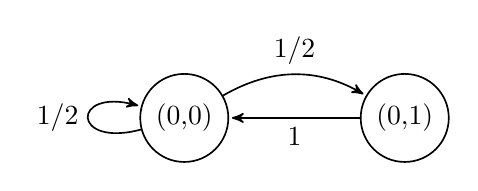
\begin{tikzpicture}[->,>=stealth',shorten >=1pt,auto,node distance=2.8cm, semithick]
          \tikzstyle{every state}=[fill=none,draw=black,text=black]
          \node[state] (A)              {(0,0)};
          \node[state]         (B) [right of=A] {(0,1)};

          \path (A) edge [bend left]  node {1/2} (B)
                    edge [loop left]  node {1/2} (A)
                (B) edge              node {1}   (A);
        \end{tikzpicture}
        \end{figure}


      \item We have a system of equations:
        $$0.5x + y = x$$
        $$0.5x + 0y = y$$
        $$x + y = 1$$
        We can easily solve this, giving us $x = \frac{2}{3}$, $y = \frac{1}{3}$, so:
        $$\pi = [\frac{2}{3},\frac{1}{3}]$$
    \end{enumerate}

  \item 
    \begin{enumerate}
      \item The number of devices in a Wi-Fi Direct group network is expected to be smaller than the number supported by traditional Wi-Fi access points.
      \item Wi-Fi Direct has speeds similar to traditional Wi-Fi, which can be as fast as 250 Mbps.
      \item Wi-Fi Direct can connect as far as 200 meters (but of course it varies, as it does with traditional Wi-Fi).
      \item Yes it can -- by creating simulataneous infrastructure and Wi-Fi Direct connections.
    \end{enumerate}
\end{enumerate}

\end{document}
